\documentclass[12pt]{article}

\usepackage{times}
\usepackage{graphicx}
\usepackage{amsmath}
\usepackage{url}

\setlength{\textwidth}{6.5in}
\setlength{\textheight}{8.9in}
\setlength{\oddsidemargin}{0.0in}
\setlength{\topmargin}{0.05in}
\setlength{\headheight}{-0.05in}
\setlength{\headsep}{0.0in}

\newcommand{\indep}{\perp\!\!\!\perp}

\begin{document}

\begin{center}
{\bf CS 6300} \hfill {\large\bf HW07: Bayes Nets I \hfill {\bf Ryan Dalby} \hfill April 5, 2022}
\end{center}

\section{D-Separation}

You missed the Artificial Intelligence Exam! When you try to explain to your professor your excuses for 
missing the exam, he stops you.  He offers to give you a grade based on your performance of mapping
your excuses and determining the D-separation of the excuses and the events associated with them. 
You draw out the events as a Bayes net seen above.  You must now answer the following questions
about the net to see what your grade for the exam you missed!

\begin{center}
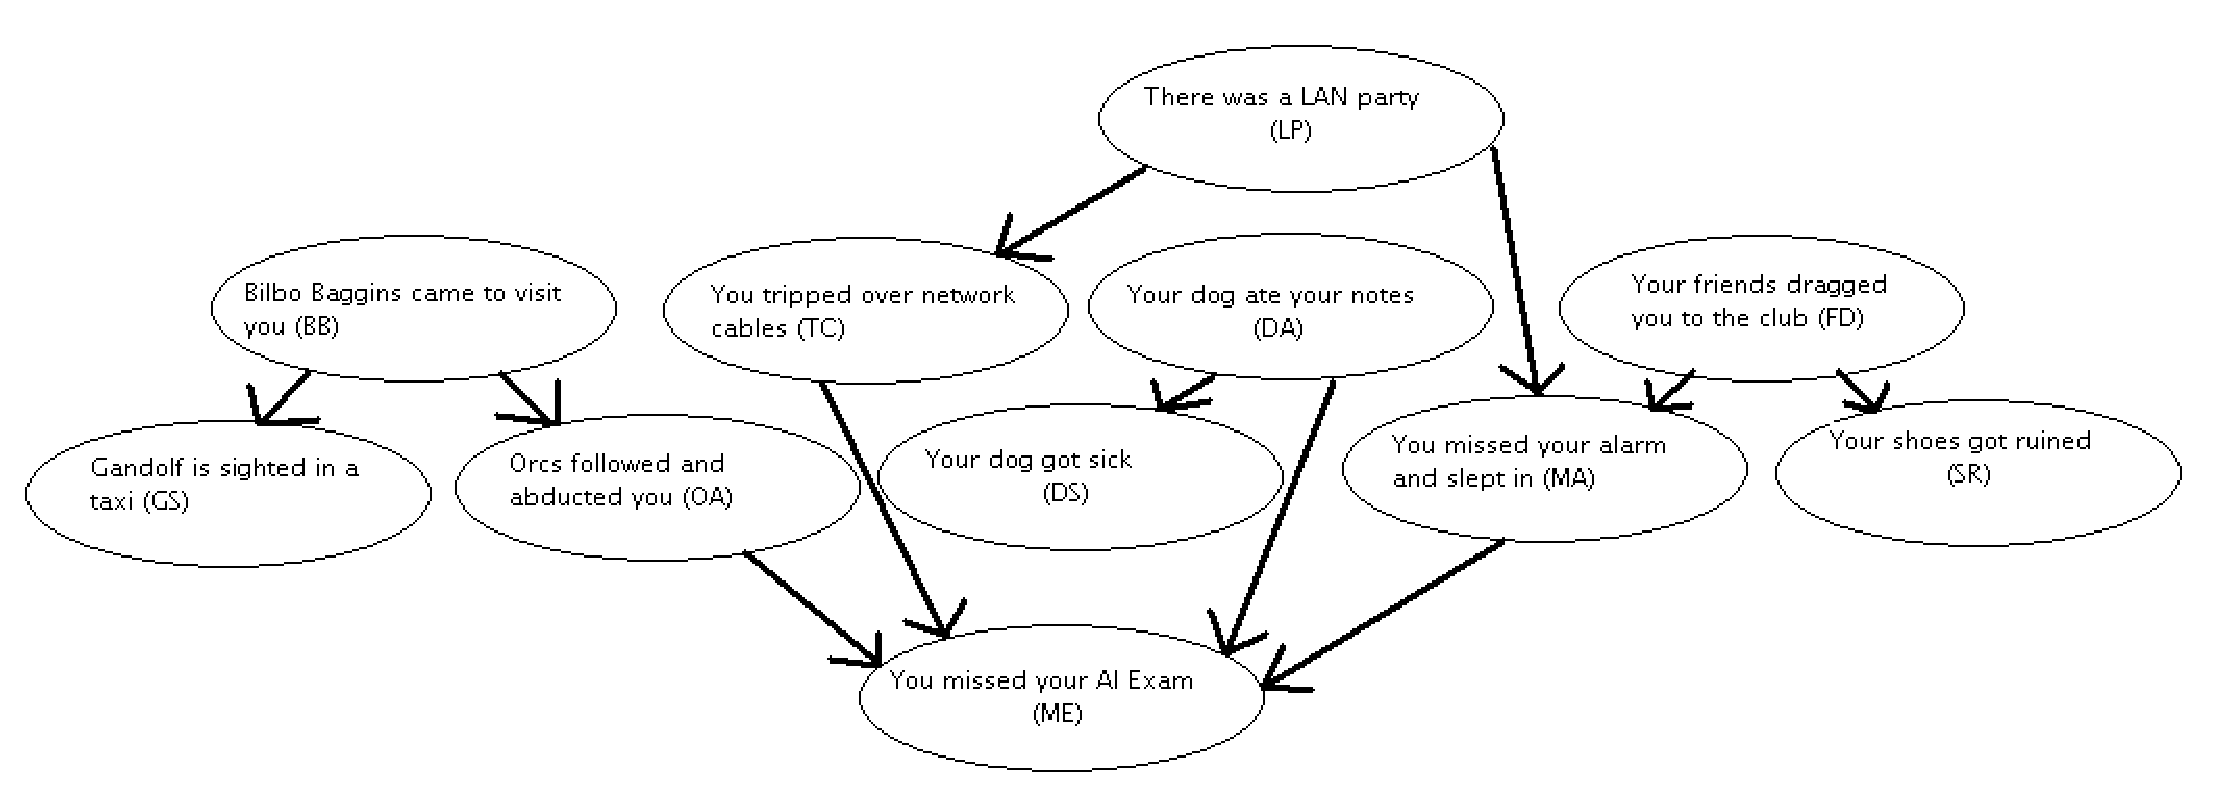
\includegraphics[width=1.0\textwidth]{excuses.eps}
\end{center}

\noindent 
Consider the following pairs of variables to answer the questions below:
\newline\newline
\centerline{(a) $GS$ and $OA$  ;  (b) $DA$ and $MA$  ;  (c) $LP$ and $FD$  ;  (d) $TC$ and $MA$  ;  (e) $BB$ and $ME$}

Given the stated evidence, list the variables that are independent or conditionally independent.

\begin{enumerate}

	\item (4 points) No information (even the evidence that you missed the exam).

	(b) and (c) are independent.

	\begin{enumerate}
		\item[a.]
		Active:
		\begin{center}
			\begin{tabular}{|c|c|c|}
				\hline
				Path & Triple & Inactive Triple? \\
				\hline
				GS,BB,OA & BB,GS,OA & No \\
				\hline
			\end{tabular}
		\end{center}

		\item[b.]
		Inactive, independent:
		\begin{center}
			\begin{tabular}{|c|c|c|}
				\hline
				Path & Triple & Inactive Triple? \\
				\hline
				DA,ME,MA & DA,MA,ME & Yes \\
				\hline
				DA,ME,TC,LP,MA & DA,TC,ME & Yes \\
				\hline
			\end{tabular}
		\end{center}

		\item[c.]
		Inactive, independent:
		\begin{center}
			\begin{tabular}{|c|c|c|}
				\hline
				Path & Triple & Inactive Triple? \\
				\hline
				LP,MA,FD & LP,FD,MA & Yes \\
				\hline
				LP,TC,ME,MA,FD & LP,TC,ME & No \\
				& TC,MA,ME & Yes \\
				\hline
			\end{tabular}
		\end{center}

		\item[d.]
		Active:
		\begin{center}
			\begin{tabular}{|c|c|c|}
				\hline
				Path & Triple & Inactive Triple? \\
				\hline
				TC,LP,MA & LP,TC,MA & No \\
				\hline
			\end{tabular}
		\end{center}

		\item[e.]
		Active:
		\begin{center}
			\begin{tabular}{|c|c|c|}
				\hline
				Path & Triple & Inactive Triple? \\
				\hline
				BB,OA,ME & BB,OA,ME & No \\
				\hline
			\end{tabular}
		\end{center}
	
	\end{enumerate}


	\item (4 points) $MA$ is observed.

	(b) is independent given the evidence.

	\begin{enumerate}
		\item[a.]
		Active:
		\begin{center}
			\begin{tabular}{|c|c|c|}
				\hline
				Path & Triple & Inactive Triple? \\
				\hline
				GS,BB,OA & BB,GS,OA & No \\
				\hline
			\end{tabular}
		\end{center}

		\item[b.]
		Inactive, independent given the evidence:
		\begin{center}
			\begin{tabular}{|c|c|c|}
				\hline
				Path & Triple & Inactive Triple? \\
				\hline
				DA,ME,MA & DA,MA,ME & Yes \\
				\hline
				DA,ME,TC,LP,MA & DA,TC,ME & Yes \\
				\hline
			\end{tabular}
		\end{center}

		\item[c.]
		Active:
		\begin{center}
			\begin{tabular}{|c|c|c|}
				\hline
				Path & Triple & Inactive Triple? \\
				\hline
				LP,MA,FD & LP,FD,MA & No \\
				\hline
			\end{tabular}
		\end{center}

		\item[d.]
		Active:
		\begin{center}
			\begin{tabular}{|c|c|c|}
				\hline
				Path & Triple & Inactive Triple? \\
				\hline
				TC,LP,MA & LP,TC,MA & No \\
				\hline
			\end{tabular}
		\end{center}

		\item[e.]
		Active:
		\begin{center}
			\begin{tabular}{|c|c|c|}
				\hline
				Path & Triple & Inactive Triple? \\
				\hline
				BB,OA,ME & BB,OA,ME & No \\
				\hline
			\end{tabular}
		\end{center}
	\end{enumerate}

	\item (4 points) $BB$ is observed.

	(a), (b), and (c) are independent given the evidence.

	\begin{enumerate}
		\item[a.]
		Inactive, independent given the evidence:
		\begin{center}
			\begin{tabular}{|c|c|c|}
				\hline
				Path & Triple & Inactive Triple? \\
				\hline
				GS,BB,OA & BB,GS,OA & Yes \\
				\hline
			\end{tabular}
		\end{center}

		\item[b.]
		Inactive, independent given the evidence:
		\begin{center}
			\begin{tabular}{|c|c|c|}
				\hline
				Path & Triple & Inactive Triple? \\
				\hline
				DA,ME,MA & DA,MA,ME & Yes \\
				\hline
				DA,ME,TC,LP,MA & DA,TC,ME & Yes \\
				\hline
			\end{tabular}
		\end{center}

		\item[c.]
		Inactive, independent given the evidence:
		\begin{center}
			\begin{tabular}{|c|c|c|}
				\hline
				Path & Triple & Inactive Triple? \\
				\hline
				LP,MA,FD & LP,FD,MA & Yes \\
				\hline
				LP,TC,ME,MA,FD & LP,TC,ME & No \\
				& TC,MA,ME & Yes \\
				\hline
			\end{tabular}
		\end{center}

		\item[d.]
		Active:
		\begin{center}
			\begin{tabular}{|c|c|c|}
				\hline
				Path & Triple & Inactive Triple? \\
				\hline
				TC,LP,MA & LP,TC,MA & No \\
				\hline
			\end{tabular}
		\end{center}

		\item[e.]
		Active:
		\begin{center}
			\begin{tabular}{|c|c|c|}
				\hline
				Path & Triple & Inactive Triple? \\
				\hline
				BB,OA,ME & BB,OA,ME & No \\
				\hline
			\end{tabular}
		\end{center}

	\end{enumerate}

	\item (4 points) $LP$ is observed.

	(b), (c), and (d) are independent given the evidence.

	\begin{enumerate}
		\item[a.]
		Active:
		\begin{center}
			\begin{tabular}{|c|c|c|}
				\hline
				Path & Triple & Inactive Triple? \\
				\hline
				GS,BB,OA & BB,GS,OA & No \\
				\hline
			\end{tabular}
		\end{center}

		\item[b.]
		Inactive, independent given the evidence:
		\begin{center}
			\begin{tabular}{|c|c|c|}
				\hline
				Path & Triple & Inactive Triple? \\
				\hline
				DA,ME,MA & DA,MA,ME & Yes \\
				\hline
				DA,ME,TC,LP,MA & DA,TC,ME & Yes \\
				\hline
			\end{tabular}
		\end{center}

		\item[c.]
		Inactive, independent given the evidence:
		\begin{center}
			\begin{tabular}{|c|c|c|}
				\hline
				Path & Triple & Inactive Triple? \\
				\hline
				LP,MA,FD & LP,FD,MA & Yes \\
				\hline
				LP,TC,ME,MA,FD & LP,TC,ME & No \\
				& TC,MA,ME & Yes \\
				\hline
			\end{tabular}
		\end{center}

		\item[d.]
		Inactive, independent given the evidence:
		\begin{center}
			\begin{tabular}{|c|c|c|}
				\hline
				Path & Triple & Inactive Triple? \\
				\hline
				TC,LP,MA & LP,TC,MA & Yes \\
				\hline
				TC,ME,MA & TC,MA,ME & Yes \\
				\hline
			\end{tabular}
		\end{center}

		\item[e.]
		Active:
		\begin{center}
			\begin{tabular}{|c|c|c|}
				\hline
				Path & Triple & Inactive Triple? \\
				\hline
				BB,OA,ME & BB,OA,ME & No \\
				\hline
			\end{tabular}
		\end{center}

	\end{enumerate}

	\item (4 points) $TC$ is observed.

	(b) and (c) are independent given the evidence.

	\begin{enumerate}
		\item[a.]
		Active:
		\begin{center}
			\begin{tabular}{|c|c|c|}
				\hline
				Path & Triple & Inactive Triple? \\
				\hline
				GS,BB,OA & BB,GS,OA & No \\
				\hline
			\end{tabular}
		\end{center}

		\item[b.]
		Inactive, independent given the evidence:
		\begin{center}
			\begin{tabular}{|c|c|c|}
				\hline
				Path & Triple & Inactive Triple? \\
				\hline
				DA,ME,MA & DA,MA,ME & Yes \\
				\hline
				DA,ME,TC,LP,MA & DA,TC,ME & Yes \\
				\hline
			\end{tabular}
		\end{center}

		\item[c.]
		Inactive, independent given the evidence:
		\begin{center}
			\begin{tabular}{|c|c|c|}
				\hline
				Path & Triple & Inactive Triple? \\
				\hline
				LP,MA,FD & LP,FD,MA & Yes \\
				\hline
				LP,TC,ME,MA,FD & LP,TC,ME & Yes \\
				\hline
			\end{tabular}
		\end{center}

		\item[d.]
		Active:
		\begin{center}
			\begin{tabular}{|c|c|c|}
				\hline
				Path & Triple & Inactive Triple? \\
				\hline
				TC,LP,MA & LP,TC,MA & No \\
				\hline
			\end{tabular}
		\end{center}

		\item[e.]
		Active:
		\begin{center}
			\begin{tabular}{|c|c|c|}
				\hline
				Path & Triple & Inactive Triple? \\
				\hline
				BB,OA,ME & BB,OA,ME & No \\
				\hline
			\end{tabular}
		\end{center}

	\end{enumerate}

	\item (4 points) $LP$  and $OA$ are observed.

	(b), (c), (d), and (e) are independent given the evidence.

	\begin{enumerate}
		\item[a.]
		Active:
		\begin{center}
			\begin{tabular}{|c|c|c|}
				\hline
				Path & Triple & Inactive Triple? \\
				\hline
				GS,BB,OA & BB,GS,OA & No \\
				\hline
			\end{tabular}
		\end{center}

		\item[b.]
		Inactive, independent given the evidence:
		\begin{center}
			\begin{tabular}{|c|c|c|}
				\hline
				Path & Triple & Inactive Triple? \\
				\hline
				DA,ME,MA & DA,MA,ME & Yes \\
				\hline
				DA,ME,TC,LP,MA & DA,TC,ME & Yes \\
				\hline
			\end{tabular}
		\end{center}

		\item[c.]
		Inactive, independent given the evidence:
		\begin{center}
			\begin{tabular}{|c|c|c|}
				\hline
				Path & Triple & Inactive Triple? \\
				\hline
				LP,MA,FD & LP,FD,MA & Yes \\
				\hline
				LP,TC,ME,MA,FD & LP,TC,ME & No \\
				& TC,MA,ME & Yes \\
				\hline
			\end{tabular}
		\end{center}

		\item[d.]
		Inactive, independent given the evidence:
		\begin{center}
			\begin{tabular}{|c|c|c|}
				\hline
				Path & Triple & Inactive Triple? \\
				\hline
				TC,LP,MA & LP,TC,MA & Yes \\
				\hline
				TC,ME,MA & TC,MA,ME & Yes \\
				\hline
			\end{tabular}
		\end{center}

		\item[e.]
		Inactive, independent given the evidence:
		\begin{center}
			\begin{tabular}{|c|c|c|}
				\hline
				Path & Triple & Inactive Triple? \\
				\hline
				BB,OA,ME & BB,OA,ME & Yes \\
				\hline
			\end{tabular}
		\end{center}

	\end{enumerate}

	\item (4 points) $ME$ is observed.

	None can be said to be independent given the evidence.

	\begin{enumerate}
		\item[a.]
		Active:
		\begin{center}
			\begin{tabular}{|c|c|c|}
				\hline
				Path & Triple & Inactive Triple? \\
				\hline
				GS,BB,OA & BB,GS,OA & No \\
				\hline
			\end{tabular}
		\end{center}

		\item[b.]
		Active:
		\begin{center}
			\begin{tabular}{|c|c|c|}
				\hline
				Path & Triple & Inactive Triple? \\
				\hline
				DA,ME,MA & DA,MA,ME & No \\
				\hline
			\end{tabular}
		\end{center}

		\item[c.]
		Active:
		\begin{center}
			\begin{tabular}{|c|c|c|}
				\hline
				Path & Triple & Inactive Triple? \\
				\hline
				LP,MA,FD & LP,FD,MA (...ME) & No \\
				\hline
			\end{tabular}
		\end{center}

		\item[d.]
		Active:
		\begin{center}
			\begin{tabular}{|c|c|c|}
				\hline
				Path & Triple & Inactive Triple? \\
				\hline
				TC,LP,MA & LP,TC,MA & No \\
				\hline
			\end{tabular}
		\end{center}

		\item[e.]
		Active:
		\begin{center}
			\begin{tabular}{|c|c|c|}
				\hline
				Path & Triple & Inactive Triple? \\
				\hline
				BB,OA,ME & BB,OA,ME & No \\
				\hline
			\end{tabular}
		\end{center}

	\end{enumerate}

\end{enumerate}

\clearpage

\section{Inference by Enumeration}

\begin{center}
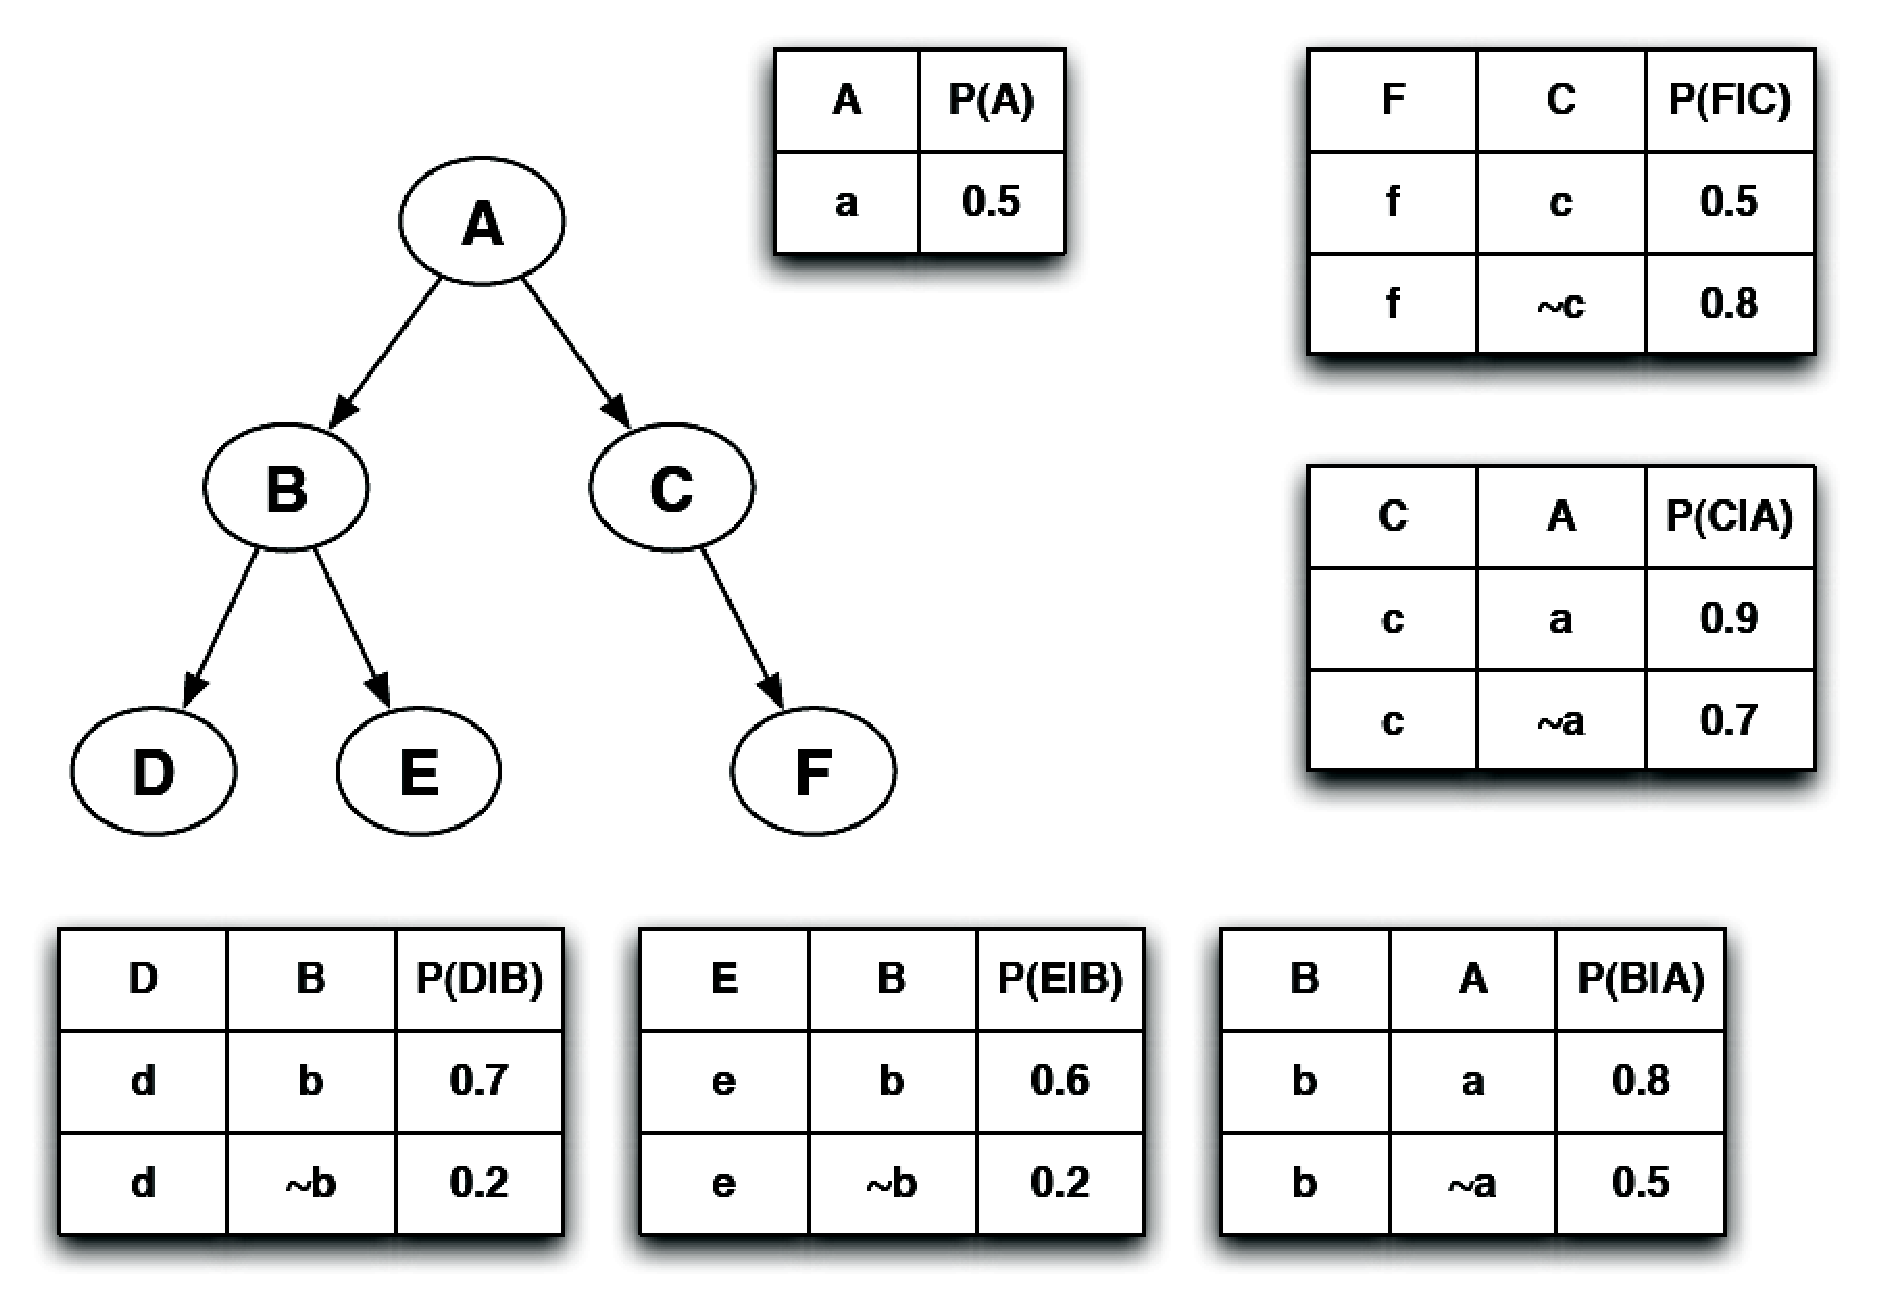
\includegraphics[width=5in]{enumeration.eps}
\end{center}

Note: for this problem I am assuming all variables $X$ can take on only two values of $x$ or $\sim x$.

\begin{enumerate}

\item What is the expression for $P(A,b,C, \sim d,E,f)$ given the structure
  of this Bayes' net and conditional probability tables?

$P(A,B,C,D,E,F) = P(A) P(B|A) P(C|A) P(D|B)P(E|B) P(F|C)$

$P(A,b,C, \sim d,E,f) = P(A) P(b|A) P(C|A) P(\sim d|b) P(E|b) P(f|C)$

% $P(A,b,C, \sim d,E,f) = P(A) P(b|A) P(C|A) (0.3) P(E|b) P(f|C)$

\item Form the joint distribution $P(A,b,C, \sim d,E,f)$ using factors.  Please give the
  details of your derivation.

$f_1(A) = P(A)$

$f_2(A,B) = f_2(A) = P(b|A)$

$f_3(A,C) = P(C|A)$

$f_4(B,D) = f_4 = P(\sim d|b) = 0.3$

$f_5(B,E) = f_5(E) = P(E|b)$

$f_6(C,F) = f_6(C) = P(f|C)$

$P(A,b,C, \sim d,E,f) = f_1(A) \times f_2(A) \times f_3(A,C) \times f_4 \times f_5(E) \times f_6(C)$

Joining on A:

$f_7(A,C) = f_1(A) \times f_2(A) \times f_3(A,C)$

\begin{center}
	\begin{tabular}{|c|c|c|}
		\hline
		$A$ & $C$ & $f_7(A,C)$ \\
		\hline
		$a$ & $c$ & $(0.5)(0.8)(0.9) = 0.36$ \\
		\hline
		$a$ & $\sim c$ & $(0.5)(0.8)(0.1) = 0.04$ \\
		\hline
		$\sim a$ & $c$ & $(0.5)(0.5)(0.7) = 0.175$ \\
		\hline
		$\sim a$ & $\sim c$ & $(0.5)(0.5)(0.3) = 0.075$ \\
		\hline
	\end{tabular}
\end{center}

Joining on C:

$f_8(A,C) = f_7(A,C) \times f_6(C)$

\begin{center}
	\begin{tabular}{|c|c|c|}
		\hline
		$A$ & $C$ & $f_8(A,C)$ \\
		\hline
		$a$ & $c$ & $(0.36)(0.5) = 0.18$ \\
		\hline
		$a$ & $\sim c$ & $(0.04)(0.8) = 0.032$ \\
		\hline
		$\sim a$ & $c$ & $(0.175)(0.5) = 0.0875$ \\
		\hline
		$\sim a$ & $\sim c$ & $(0.075)(0.8) = 0.06$ \\
		\hline
	\end{tabular}
\end{center}

Then finally forming the factor that is equivalent to the desired expression:

$P(A,b,C, \sim d,E,f) = f_9(A,C,E) = f_8(A,C) \times f_4 \times f_5(E) = f_8(A,C) \times (0.3) \times f_5(E)$

\begin{center}
	\begin{tabular}{|c|c|c|c|}
		\hline
		$A$ & $C$ & $E$ & $P(A,b,C, \sim d,E,f)$ \\
		\hline
		$a$ & $c$ & $e$ & $(0.18)(0.3)(0.6) = 0.0324 $ \\
		\hline
		$a$ & $c$ & $\sim e$ & $(0.18)(0.3)(0.4) = 0.0216$ \\
		\hline
		$a$ & $\sim c$ & $e$ & $(0.032)(0.3)(0.6) = 0.00576$ \\
		\hline
		$a$ & $\sim c$ & $\sim e$ & $(0.032)(0.3)(0.4) = 0.00384$ \\
		\hline
		$\sim a$ & $c$ & $e$ & $(0.0875)(0.3)(0.6) = 0.01575$ \\
		\hline
		$\sim a$ & $c$ & $\sim e$ & $(0.0875)(0.3)(0.4) = 0.0105$ \\
		\hline
		$\sim a$ & $\sim c$ & $e$ & $(0.06)(0.3)(0.6) = 0.0072$ \\
		\hline
		$\sim a$ & $\sim c$ & $\sim e$ & $(0.06)(0.3)(0.4) = 0.0108$ \\
		\hline
	\end{tabular}
\end{center}

\item Solve for the query $P(C | b, \sim d, f)$.

\[
	P(C | b, \sim d, f) = \frac{P(C, b, \sim d, f)}{P(b, \sim d, f)} = \alpha P(C, b, \sim d, f)
\]

where $\alpha$ is a constant

\[
	P(C, b, \sim d, f) = \sum_A \sum_E P(A,b,C, \sim d,E,f)
\]
\begin{center}
	\begin{tabular}{|c|c|c|}
		\hline
		$A$ & $C$ & $P(A,b,C, \sim d,E,f)$ \\
		\hline
		$a$ & $c$ & $0.054$ \\
		\hline
		$a$ & $\sim c$ & $0.0096$ \\
		\hline
		$\sim a$ & $c$ & $0.02625$ \\
		\hline
		$\sim a$ & $\sim c$ & $0.018$ \\
		\hline
	\end{tabular}
\end{center}

\[
	P(C, b, \sim d, f) = \sum_A P(A,b,C, \sim d,f)
\]

\begin{center}
	\begin{tabular}{|c|c|}
		\hline
		$C$ & $P(C,b,\sim d,f)$ \\
		\hline
		$c$ & $0.08025$ \\
		\hline
		$\sim c$ & $0.0276$ \\
		\hline
	\end{tabular}
\end{center}

Now using the laws of probability, $\alpha = \frac{1}{0.08025 + 0.0276} = 9.272$

\begin{center}
	\begin{tabular}{|c|c|}
		\hline
		$C$ & $P(C|b,\sim d,f)$ \\
		\hline
		$c$ & $0.744$ \\
		\hline
		$\sim c$ & $0.256$ \\
		\hline
	\end{tabular}
\end{center}

\end{enumerate}

\end{document}


